\chapter{Conceptual design}\label{chap:concept}
Using the knowledge from the literature survey we start by designing a general concept of the distance sensing system. Focus is put on the trade offs and design decisions made during the first part of the project. We will first discuss the general concept after which we will go into more detail on the subsystems. We will discuss what is required of these subsystems and provide different options to obtain the required functionalities. The most suitable options is selected, where necessary, and an implementation is given. The chosen implementations are validated using simulations. At the end of this chapter we will have implementations of the subsystems that can be used for the proof of concept. Focus is put on the working of the subsystems. The integration of the subsystems with each other and with the other systems in the module, communication and processing, will be discussed in the prototype design.

\section{Concept}

Based on the literature survey we decide to base our design on the MIT cricket system. We want to use an RF message in combination with an ultrasonic pulse to get an accurate estimation of the distance between multiple Zebros. Due to the propagation speed difference of sound waves and EM waves we get an time difference of arrival (TDOA) when the two signals are transmitted at the same time. Since, over these small distances, the RF message arrives almost instantly we can set the moment the RF signal arrives as $t_{0}$. At $t_{0}$ we start a time to measure the time it takes for the ultrasonic pulse to reach to receiver ($\Delta t$). Since the ultrasonic pulse travels at the speed of sound we can express the distance (D) between sender and receiver in the time difference $\Delta t$ and the propagation velocity of sound $V_{sound}$.\\

$ D = V_{sound} * \Delta t $\\

An advantage is that, when the ultrasonic pulse is transmitted in all directions all Zebros within range will receive both the RF message and the ultrasonic pulse giving them enough information to determine the distance between themselves and the transmitting Zebro which complies to requirement~\ref{req:neighbours}.
The RF message will include a Zebro identifier tag so the receivers can distinguish the different Zebros in the swarm which complies to requirement~\ref{req:distinguish}.

\begin{figure}[H]
\centering
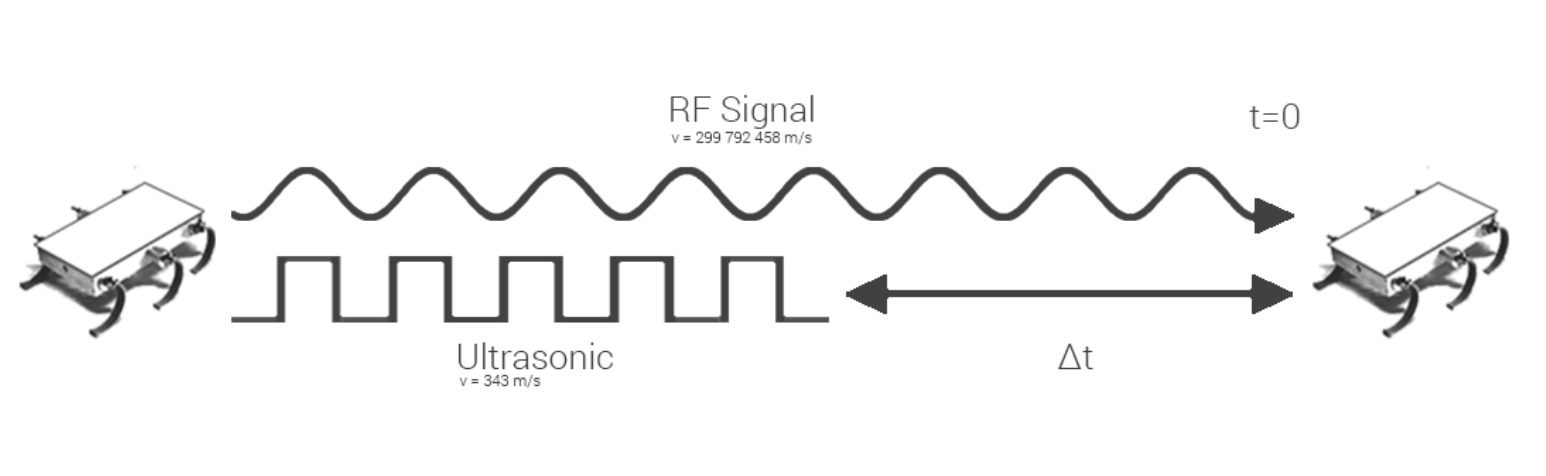
\includegraphics[width=0.8\textwidth]{Figures/Rf_vs_Us.jpeg}
\caption{TDOA of RF message and ultrasonic pulse}\label{fig:ultra1}
\end{figure}

Because the range of the RF message is easily 3 times the range of the ultrasonic pulse, which can be further limited by the receiving circuit, a Zebro will never receive an ultrasonic pulse without the accompanying RF message. Furthermore the RF message is hopped trough the Zebro swarm making sure that the message reaches all Zebros.

\begin{figure}[H]
\centering
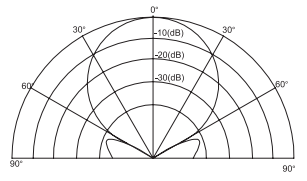
\includegraphics[width=0.5\textwidth]{Figures/ultrasonics_transceivers.PNG}
\caption{Directivity of an ultrasonics transducer}\label{fig:ultra2}
\end{figure}

%----------------------------------------------------------------------------------------
%	Tade-off
%----------------------------------------------------------------------------------------

\section{Concept implementations}
In this section we're going to look at the options to implement the concept. A comparison between the different options is made, where necessary with a criteria trade-off. Furthermore we will discuss the options for the implementation of the ultrasonic transducers, the transmitter circuit and the receiver circuit.

\subsection{Ultrasonic transducers}

One problem arises: Ultrasonic transducers don't send omnidirectional, they have a narrow beam width.
Most available transducers have a beam angle of \SI{50}{\degree} to \SI{80}{\degree}, far from the \SI{360}{\degree} we need to comply to requirement~\ref{req:omnidir}.
Two possible solutions are considered: using multiple transducers to implement a \SI{360}{\degree} transducer array or creating a omnidirectional antenna to shape the directivity of a single transducer.

We make the design trade-off based on a set of design criteria: cost, power consumption, size, precision, angle of arrival (AOA) measurements.
A system using multiple transducers would need between 4 to 8 sensors to create an omnidirectional array while the antenna systems needs a single transceiver.

\begin{table}[H]
\centering
\begin{tabular}{|l|c|c|}
    \hline
    Criteria            & Omnidirectional   & Sensor array \\
    \hline
    Cost                & ++ & -  \\
    Power consumption   & + & - \\
    Size                & - & - \\
    Range               & - & + \\
    Accuracy            & - & - \\
    AOA detection       & - & (+) \\
    \hline
\end{tabular}
\caption{Criteria comparison}
\label{tab:ant_crit}
\end{table}


\begin{itemize}
    \item
      \textbf{Cost:} The estimated cost of an ultrasonic transceiver is \euro{3} for a \SI{50}{\degree} beam width model and \euro{5} for a \SI{80}{\degree} beam width model.
      For the antenna the entire beam has to be incident on the lens of the antenna so a sensor with a small beam width (focused on the lens) is preferred.
      The antenna system needs a single transceiver since the antenna can both transmit and receive ultrasonic waves.
      The production cost of the 3D printed antenna is estimated at \euro{2}.
      The total cost would be \euro{5} plus the cost of a driver and receiver circuit.
      For the array we need at least 4 times the \SI{80}{\degree} sensors or 7 times the \SI{50}{\degree} sensors costing roughly \euro{20}.
      Furthermore we need an structure to hold the sensors at the correct angles an multiple versions of the driver and receiver circuit increasing the cost. This means the antenna systems is roughly a fifth of the price of the sensor array.
    \item
      \textbf{Power consumption:} The array would use x times the power of the antenna system where x is the number of sensors in the array.
    \item
      \textbf{Size:} The antenna system would need an exterior reflecting located on top of the system while the array systems needs more space on the circuit board, since it uses multiple drive and receiver circuits, increasing the internal space needed to house the electronics.
      Since the module is located on top of the Zebro an increase in required internal space requires a higher module so we assume that the space needed for both systems is roughly the same.
    \item
      \textbf{Range:} Since the array uses a direct configuration the received power will be higher than that off the antenna system where the waves are reflected by the lens.
      The traversed path with the antenna system is longer since the waves have to travel the extra distance to the lens and the waves are reflected in a \SI{360}{degree} pattern so that a large part of the power does not arrive at the receiver.
    \item
      \textbf{Accuracy:} We assume that there is no accuracy difference between the two systems since both only transmit a short ultrasonic pulse.
      If the ultra sonic signal would have contained information this would be distorted by the reflecting antenna.
      The only difference we expect is a time offset resulting from the extra distance the ultra sonic pulse has to travel in the antenna system. This offset is constant so easily compensated.
    \item
      \textbf{AOA detection:} An array of ultrasonic sensors gives us the possibility of calculating the AOA by comparing the difference in TOA or received power of the different sensors.
      We can estimate the same angle with the correct filter technique, as discussed in \cite{processing}, this makes the AOA capabilities of the array redundant.
\end{itemize}

Based on the criteria comparison we choose to design a distance sensing system which uses an antenna to create an omnidirectional beam pattern. This system uses a single ultrasonic transducer which can act as both a transmitter and receiver. To operate this transducer we need a switching circuit which allows us to select transmitter or receiver mode. In transmitter mode the microcontroller will generate a PWM pulse at 0-5V. This PWM pulse is amplified to generate the pulse necessary to drive the ultrasonic transducer. In receiver mode the signal detected by sensor is first amplified and then processed by a detector circuit. This detector circuit will give a high output when no signal is detected and a low output when the sensor detects a signal. The microcontroller can detect the change from high to low to determine when the ultrasonic pulse is received. The detector signal is high when there is no signal so that the system can check if the receiver section is working properly. When the systems switches to receiving mode but doesn't detect a high detection signal the microcontroller knows that there is a problem in the receiver section. An overview of this concept is given in figure ~\ref{fig:ultra3}. In the next subsections we will discuss the possible implementations of the required transmitter and receiver circuit.

\begin{figure}[H]
\centering
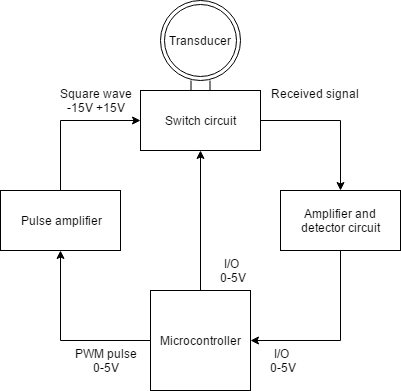
\includegraphics[width=0.6\textwidth]{Figures/concept.png}
\caption{Block diagram of distance sensing system}
\label{fig:ultra3}
\end{figure}

\subsection{Transmitter}
\label{chap:trans}

To transmit a ultrasonic signal the transducer needs to be driven by a \SI{40}{\kilo\hertz} wave.
Typical voltage levels for this wave are between $5V_{p-p}$ and $40V_{p-p}$ and is symmetrical around 0 ($V^{+}=-V^{-}=\frac{1}{2}V_{p-p}$).
We discuss 2 options to generate the \SI{40}{\kilo\hertz} \SI{50}{\percent} duty cycle wave: an operational amplifier circuit and a H-bridge driver circuit.

The operational amplifier circuit uses a comparator with supply voltage ($V^{+}=\frac{1}{2}V_{p-p}$) and ($V^{-}=-\frac{1}{2}V_{p-p}$).
When the input signal of the comparator, a \SI{50}{\percent} PWM generated by the micro controller, is above a certain threshold $V_{th}$ the output is $V^{+}$.
When the input is below $V_{th}$ the output of the comparator is $V^{-}$.
The threshold is set at half the amplitude of the PWM generated by the micro controller (typical 5V).
Since the battery output is a positive voltage \ref{req:volt} we need to create the negative supply voltage inside the module.
MIT uses an IC in their ultrasonic transmitter driver circuit that converts the VCC power supply to an $V^{+}$ and a $V^{-}$ to power the operational amplifier.
However, this IC is relatively expensive in SMD design package.

H-bridge driver circuits are typically used for motor driving circuits but, with the right selection of components, can be adapted to drive a ultrasonic transducer.
The H-bridge switches the polarity off the voltage on the ultrasonic transducer generating a PWM driving signal.
The amplitude of this signal is the supply voltage of the H-bridge.
The circuit does not require a negative supply voltage but needs 2 control waveforms which are the logic inverse of each other.
These control waveforms need to be generated by the micro controller directly or trough an inverter circuit.

Since we are not sure which solution will give the best transmitting results, we will test both circuit solutions. The first solution, the op-amp circuit, is relatively expensive because of the voltage converter, but we are sure this will work because it is already proofed on with the Cricket circuit. The H-bridge driver is typically used to drive motors so we are not sure if this will also work to drive ultrasonic transceivers. The results of H-bridge circuit will be discussed in section \ref{sec:transcircuit}.

\subsection{Receiver}
\label{chap:receiver}

The receiver circuit needs to detect if an ultrasonic signal is present.
When it receives an ultrasonic pulse it's output ($US_{detect}$) will go low allowing the microcontroller to determine at which point in time the pulse reached the ultrasonic transducer.
The MIT Cricket indoor location system \cite{Balakrishnan2003, Priyantha2000} project has used two types of detection circuits: A phase-locked loop (PLL) in combination with a tone detector and as a second option an amplitude detection circuit.
Before the detector circuits are able to detect an ultrasonic pulse the received signal needs to be amplified.

The PLL detector generates a output signal whose phase is related to the phase of the input signal.
This means that the frequency of the output signal is the same as the frequency of the input signal.
Since the frequency of the ultrasonic pulse is known to be \SI{40}{\kilo\hertz}
the signal can be recovered from the ultrasonic transducer.
The output of the PLL will then be a signal with a frequency of \SI{40}{\kilo\hertz} when the transducer receives an ultrasonic pulse.
The signal will then be presented to a tone detector which detects if the signal has a frequency of \SI{40}{\kilo\hertz} or not.
The output of this tone detector is high when the frequency of it's input is not \SI{40}{\kilo\hertz}, which corresponds to not receiving an ultrasonic pulse, and low when the frequency of it's input is \SI{40}{\kilo\hertz} corresponding to receiving an ultrasonic pulse.

The second solution, the amplitude detector, uses a peak detection circuit to detect the amplified received signal.
The peak detection circuit consists of a diode, a capacitor and a resistor as pictured in \ref{fig:peak_d}.
The signal on the input of the detector charges the capacitor.
When the ultrasonic transducer doesn't receive a signal the amplified received signal will be a DC voltage.
In this case the output of the detector circuit will be the input DC voltage.
When the transducer does receive an ultrasonic signal the input will be a biased sinusoidal wave.
The bias of this sinusoidal wave is the DC voltage present when the systems doesn't receive an ultrasonic signal.
Now the capacitor is charged by the sinusoidal wave and discharges over the resistor.
The capacitor charges due to this sinusoidal wave, the voltage over the capacitor basically follows the input voltage source. It will charge up to the peak voltage of the signal. Once it reaches this voltage, the capacitor discharges over the resistor.  It does not discharge back through the diode because the diode is a one-way current device. The voltage across the capacitor isn't directly the peak voltage of the waveform. This is because the diode consumes some voltage. Therefore the maximum voltage measured across the output is actually higher than the input voltage by a factor of the voltage drop across the diode. To get the true peak voltage, we must subtract the voltage that the diode consumes from the output signal.
So if we measure the voltage at the capacitor to be 9V and the diode consumes 0.6V, the peak voltage of the input signal is actually 8.4V. The time it will take for the capacitor to completely discharge is 5RC, where R is the resistance and C is the capacitance. This time needs to be larger than the time of a half period of the 40 kHz signal, which is 0.0125 $ms^{-1}$. So the RC need to be larger than $5 * 0,0125 ms^{-1} = 0.0625$. \footnote{The final values differ from the given RC value. This is due the non ideal behaviour of physical capacitors. The final values as given in the circuit \ref{Appendixcircuits} are found by testing different configurations on a breadboard.} With this RC the capacitor discharges slowly enough to have a signal so the comparator can detect the difference between a received and not received signal.

\begin{figure}[H]
\centering
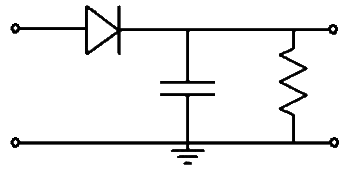
\includegraphics[width=0.4\textwidth]{Figures/peak_d.PNG}
\caption{Peak detection circuit}
\label{fig:peak_d}
\end{figure}

The first version of the MIT Cricket indoor localisation system used a PLL to detect the ultrasonic signal \cite{Priyantha2000}.
In \cite{Balakrishnan2003} the lessons learned from Cricket V1 and explain that the PLL system had highly variable detection characteristics leading to high measurement errors.
They have since then implemented a amplitude detection circuit and found it to improve detection accuracy.
Using this knowledge we opt to design our own peak detection system instead of a PLL.

\section{Antenna design}
The first thing that is considered is the shape of the ultrasonic reflecting antenna. An optimised design is not in the scope of this projects so we will be basing our design on three basic antenna shapes: cone, sphere and parabolic.

\begin{figure}[H]
\centering
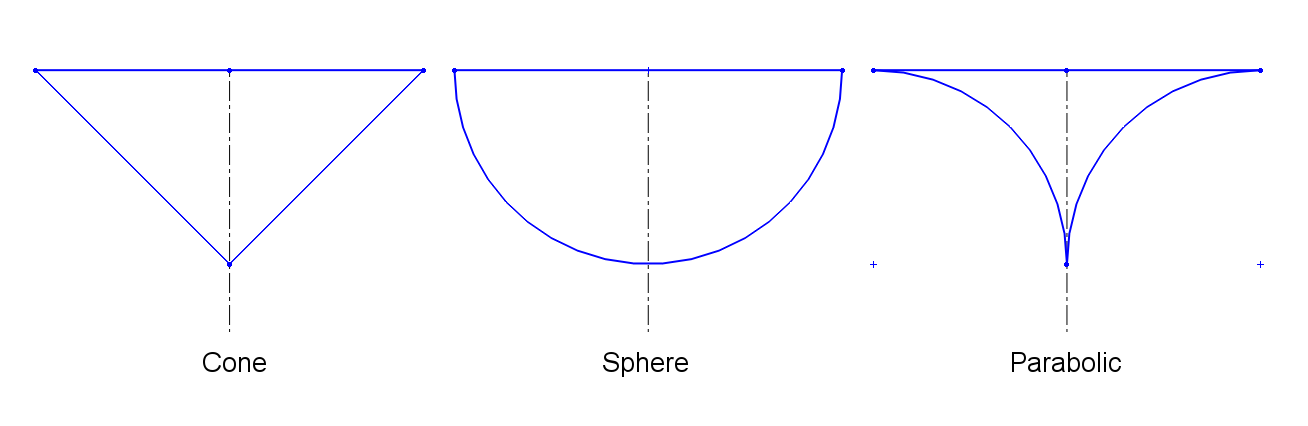
\includegraphics[width=0.9\textwidth]{Figures/ant_shapes.PNG}
\caption{Possible shapes for the reflector antenna, the cone, the sphere and the parabolic design}
\label{fig:shapes}
\end{figure}

Requirements for the antenna are is:

\begin{enumerate}[label={[A.\arabic*]}]
  \item
  \textbf{Transmitting and receiving:} The antenna should be usable in both a transmitting and a receiving configuration. All robots will be fitted with the same antenna and will be using a single ultrasonic transducer. \label{ref:T_R}
  \item\label{ref:a2}
  \textbf{Lightweight:} The antenna should be lightweight because it will be mounted on top op the Zebro. For stability a low centre of mass favourable.
  \item\label{ref:a3}
  \textbf{Mass production:} It has to be possible to produce the final design in large quantities.
  \item
  \textbf{Stable:} Movement of the Zebro should not change the transmitting/receiving behaviour due to movement of components in the antenna.
\end{enumerate}

To comply to requirement \ref{ref:a2} and \ref{ref:a3} we decide to produce the antenna from plastic. It's lightweight, can be produced an mass by making moulds and reflects ultrasonic waves.
The prototype will be 3D printed since the initial costs for making a mould are high and the prototype series will consist of only 5 antennas.

An numerical design for such an antenna is not in the scope of this project so we will use a wave reflection simulation tool to select the most suitable antenna shape.
Figure~\ref{fig:shapes} shows the antenna shapes we will simulate.
The figure shows half of the shape where the dotted line is the central axis of the reflector antenna.
The ultrasonic transducer will be centred on the central axis of the antenna below the reflecting surface such that the system is symmetrical.

After the simulations we will design a proof of concept version of the selected antenna.
The design of this proof of concept antenna is discussed in section ~\ref{sec:antenna_proof}.

\section{Transmitter circuit design}
\label{sec:transcircuit}

For the design of the transmitter circuit, there are two possible solutions as discussed in section \ref{chap:trans}. The first solution is the operational amplifier circuit, and the second solution is the H-bridge driver circuit.

The idea for the operational amplifier circuit is from the MIT ultrasonic transmitter driver circuit \cite{Priyantha2005}. MIT uses an IC that converts the VCC power supply to an $V^{+}$ and a $V^{-}$ to power the operational amplifier. However, this IC is relatively expensive in SMD design package. The circuit is simple because it can be driven directly out of an I/O pin of the micro controller. The signal out of the micro controller is than compared to a DC value, $V_{th}$, set on the negative pin of the operational amplifier. In this configuration the operational amplifier works as a comparator. A value on the plus pin above $V_{th}$ results in an output of $V^{+}$ and a value underneath $V_{th}$ result is an output of $V^{-}$. If the op-amp is driven with a PWM with duty cycle of 50\% and a $V_{th}$ of $\frac{1}{2}V_{p-p}$ of the I/O pin, the output of the op-amp will be symmetrical around 0 and have a wave with amplitude of $2 * V^{+}$. These outputs are desired to drive the ultrasonic transceiver.

In figure \ref{fig:h_bridge} is a typical H-bridge circuit visible. The ultrasonic transceiver is placed over the connectors J1 and J2. If signal S1 is high, J1 is connected to $VCC$ and if S2 is low, J2 will be connected to ground. Let's say this is the forward mode. The reverse mode is when S2 is high and S1 is low, than J1 is connected to ground and J2 is connected to $VCC$. In this way the ultrasonic transceiver is driven with a $V_{p-p}$ of $2 * VCC$ using only one positive power source. The output signal over J1 and J2 is symmetrical around 0 if S1 and S2 are driven with a PWM with a duty cycle of 50\%. This are, again, the desired outputs to drive the ultrasonic transceiver. The H-bridge solution seems more legit since it only uses one $VCC$ power source and no voltage converter IC in front.

\begin{figure}[H]
\centering
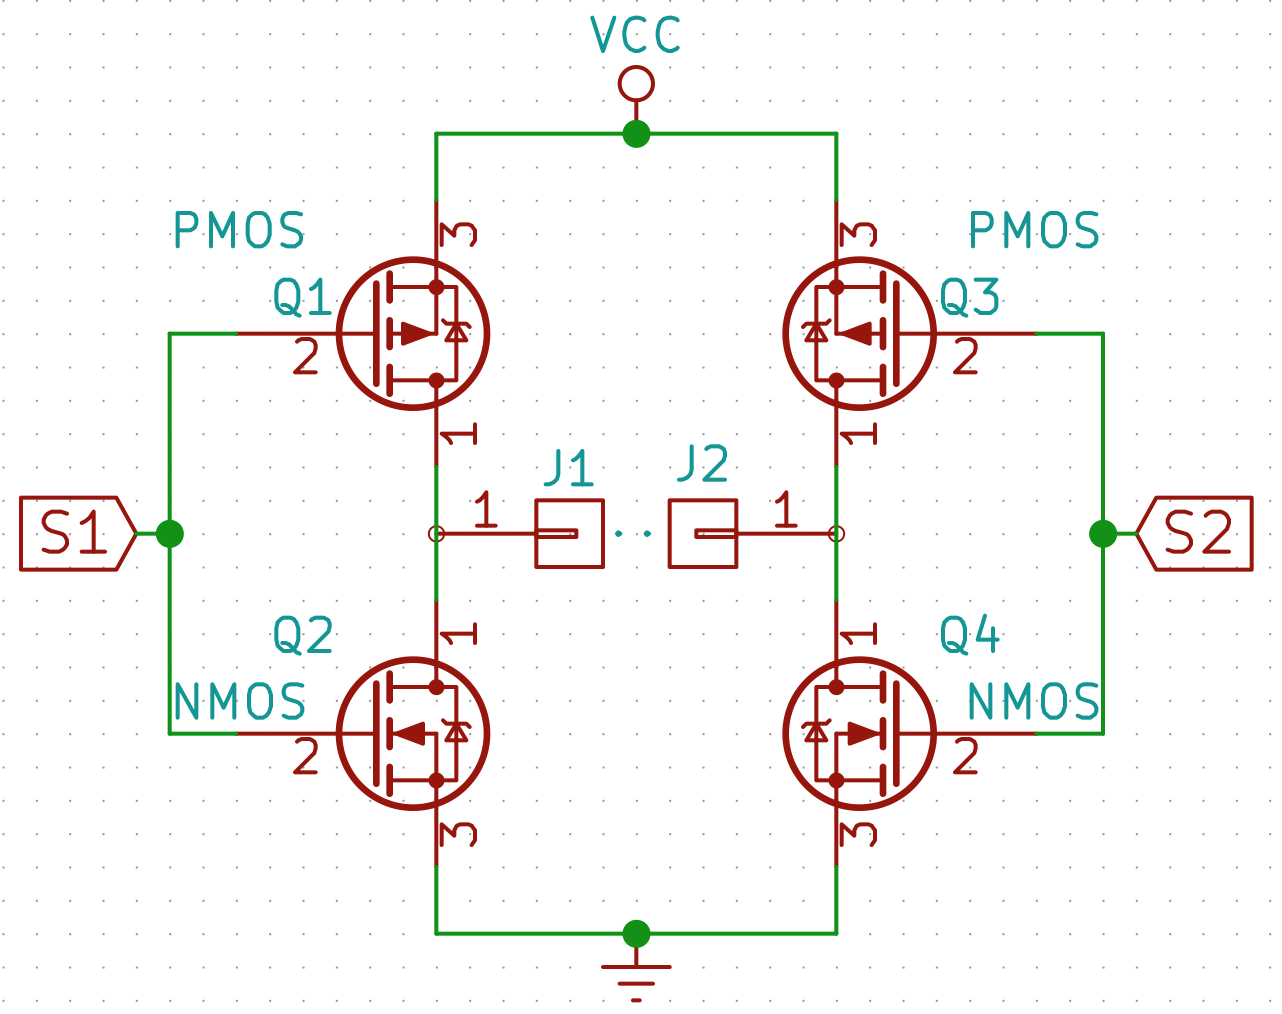
\includegraphics[width=0.6\textwidth]{Figures/hbridge.PNG}
\caption{H-bridge circuit}
\label{fig:h_bridge}
\end{figure}

To get a 30 $V_{p-p}$ PWM signal, with frequency of 40 kHZ, on the ultrasonic transceiver the $VCC$ needs to be 15V. But if the $VCC$ is 15V the MOSFET's can't be turned on and off directly out of the I/O pins of the micro controller. This is why the H-bridge needs to have a high side driver circuit, or IC, in front. After all we found an IC, the MIC4428 \cite{MIC4428}, that has typical applications to drive piezoelectric transducers and have a driver and H-bridge circuit integrated.

\section{Receiver circuit design}
\label{chap:receivercircuit}
For the receiver circuit design there were two types of detection circuits discussed before in section \ref{chap:receiver}. But regarding the conclusions of Cricket V1 we chose to use the peak detection circuit in stead of the phase lock loop detector circuit.

The ultrasonic transceiver can receive 40 kHz signals, also known as ultrasonic signal. These received signals have a very low amplitude, this is why the detection circuit needs to have an amplification. The amplification can be done using an operational amplifier. Literature study showed that one stage amplification gives a to low amplification, this is why we use a two stage operational amplification. As can be seen in figure \ref{fig:receivecircuit} the op-amps U2A and U2B are the two stages for the amplification.
The ultrasonic transceiver is connected to 1Y1 and 1Y2, as can be seen in in the figure \ref{fig:receivecircuit}. The ultrasonic transceiver is biased at a voltage of half the supply voltage of the first two stages, in this design it is $4.5V$, since we power the op-amps with $9V$. This is because the signal received on the ultrasonic transceivers is symmetrical around 0 which holds that is also receives negative voltages, but since we only power the op-amps with a positive voltage and ground we biased the ultrasonic transceiver. In this way we amplify both the positive and negative received amplitudes of the signals. The configuration in which the first two stages are used is called the differential amplifier configuration. In the feedback loops of the op-amps are pot meters visible, this is to tune the amplification of both op-amp stages.

\begin{figure}[H]
\centering
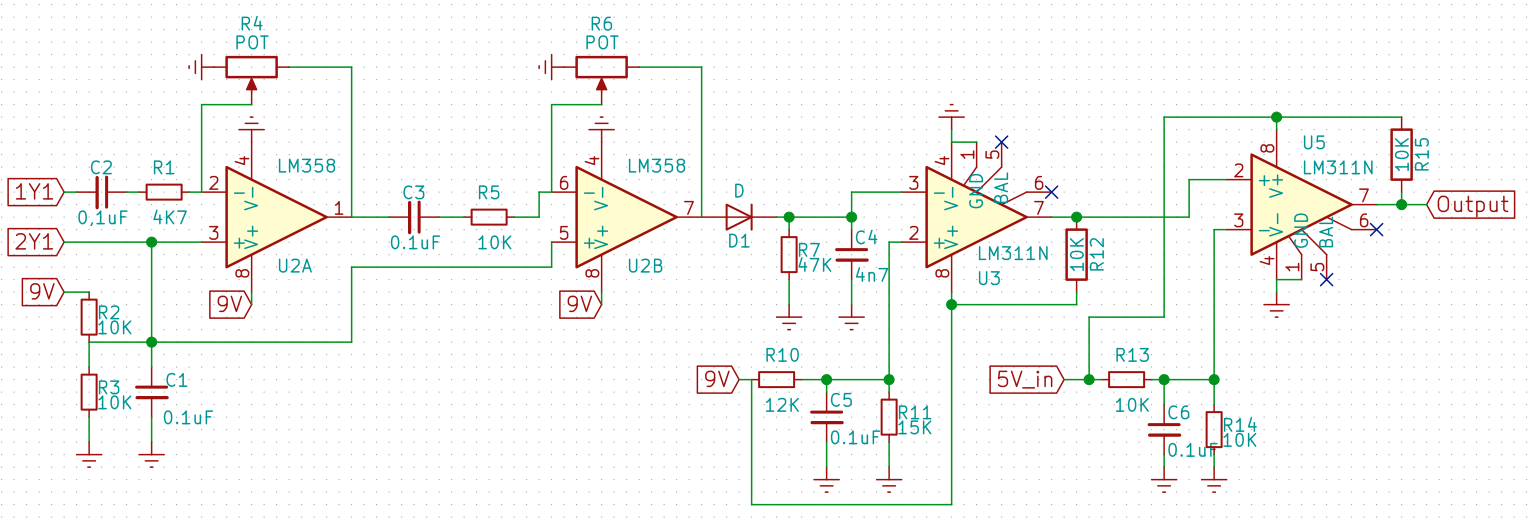
\includegraphics[width=0.9\textwidth]{Figures/receivercircuit.PNG}
\caption{The receiver circuit for the ultrasonic transceiver}
\label{fig:receivecircuit}
\end{figure}

A simple simulation that visualises what happens when the ultrasonic transceiver is not biased is visible in figure \ref{fig:nonbias}.
And a simulation where the ultrasonic transceiver is biased by half the power of the op-amp is visible in figure \ref{fig:bias}
We can conclude form these figures that it is better to bias the transceiver if we only power the operational amplifiers with a positive voltage and ground. Because with the non biased configuration, half of the signal information is thrown away.

\begin{figure}[H]
\centering
\begin{subfigure}{.5\textwidth}
  \centering
  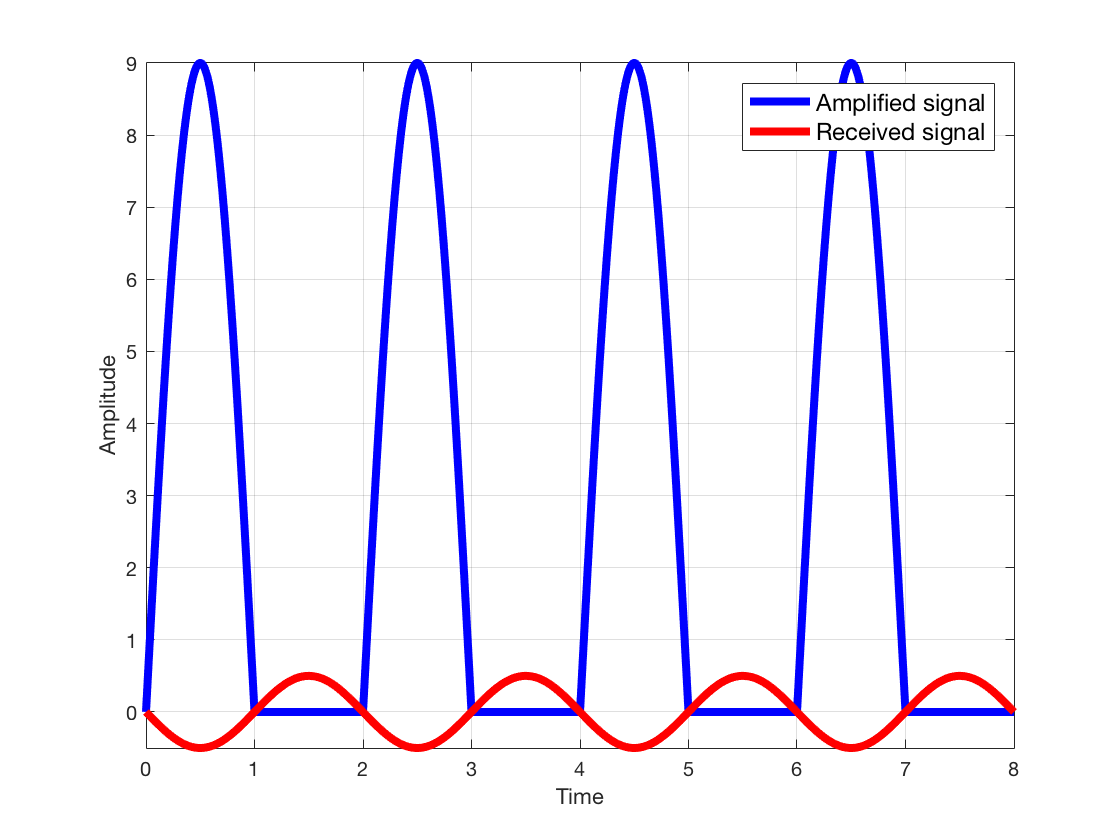
\includegraphics[width=1.0\textwidth]{Figures/nonbias.PNG}
  \caption{A simultion with no bias voltage}
  \label{fig:nonbias}
\end{subfigure}%
\begin{subfigure}{.5\textwidth}
  \centering
  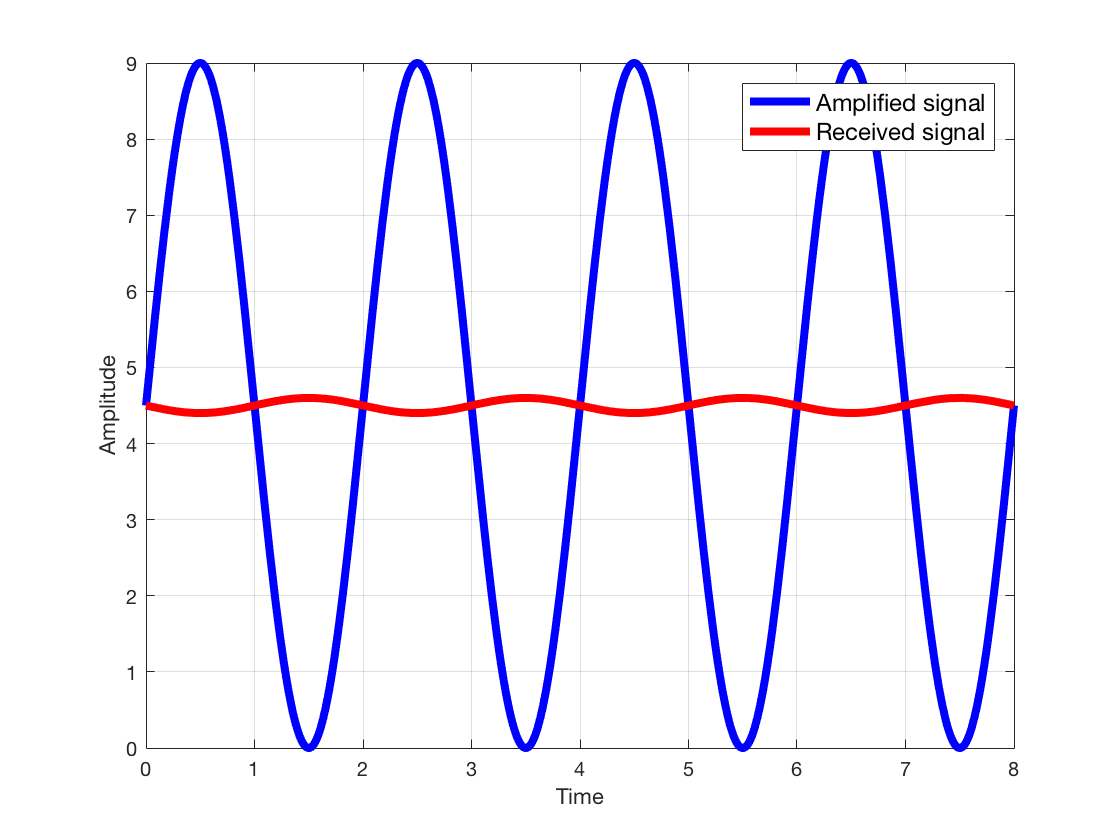
\includegraphics[width=1.0\textwidth]{Figures/bias.PNG}
  \caption{A simultion with bias voltage}
  \label{fig:bias}
\end{subfigure}
\caption{Bias simulations for the ultrasonic transceiver}
\label{fig:simulationsbias}
\end{figure}

After the two stages of amplification, the peak detection circuit is visible in figure \ref{fig:receivecircuit}. The peak detection circuit consists of a diode D1, a resistor R7 and a capacitor C4. The peak detection circuit is already mentioned before in section \ref{chap:receiver}. The desired output of the peak detection is visible in figure \ref{fig:waves_peak_detect} as the V receiving signal, the signal when not receiving an ultrasonic signal is $4.5V$ since the + pin of the op-amps of the first and second stages are kept at $4.5V$.
After the peak detection circuit, a comparator is visible in figure \ref{fig:receivecircuit}. This comparator compares the signal on the - pin of U3 to the DC value, $V_{th}$, put on the + pin of U3. This $V_{th}$ needs to be chosen to sit in between the value of the not receiving voltage and the minimum value of the receiving signal voltage on the input of the comparator, this is visible in figure \ref{fig:waves_peak_detect}. The comparator is in the circuit because we want to detect a falling edge when the ultrasonic transceiver receives a ultrasonic pulse.

The last comparator stage in the circuit makes the signal output an output that is between the desired voltages for the micro controller, 0 and 5 volt. Directly powering the first comparator stage of U3 with $5V$ could also result in an output between 0 and 5 volt, but since the $V_{th}$ is close to the supply voltage of the comparator is this not allowed.

In the rest of the circuit are some stabilisation capacitors visible to stabilise the voltages put on several pins. The capacitors C2 and C3 give the operational amplifiers an active high pass filter. The cut off frequency can be calculated with equation \ref{eq:cutof}
The first stage cut off frequency is 338.6 Hz and the cut off frequency of stage two is 159.2 Hz
\begin{equation}
\label{eq:cutof}
F_{c}= \frac{1}{2\pi RC}
\end{equation}

\begin{figure}[H]
\centering
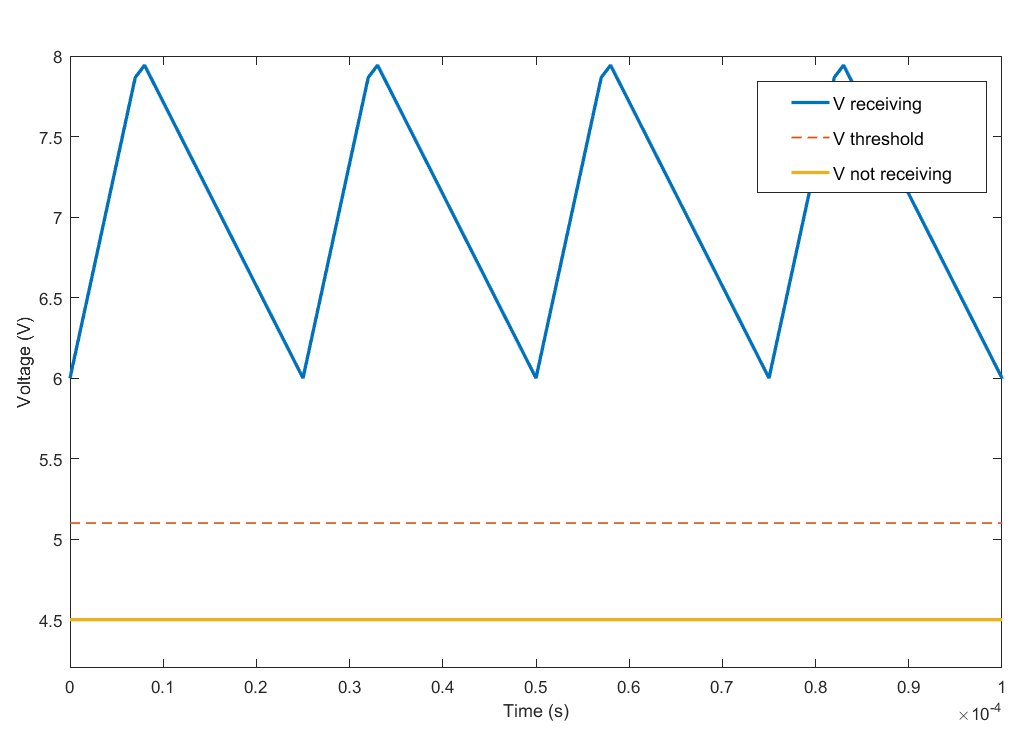
\includegraphics[width=0.5\textwidth]{Figures/waves_peak_detect.png}
\caption{Desired output peak detect circuit}
\label{fig:waves_peak_detect}
\end{figure}

\section{Simulations}

\subsection{Antenna}

Using an simulation tool \cite{Ultratool} we were able to simulate the different antenna lens shapes.
The tool is originally designed for optics but it's suitable to simulate the far field behaviour of sound waves.
Below the results of the simulations are given and discussed.
We will first look at the transmitting behaviour of the different shapes.
The most suitable shape for our application is selected.
Last we simulate the receiving behaviour of the selected shape to see if we comply to requirement \ref{ref:T_R}.

For the simulation we simulated the ultrasonic transducer by placing a point source in an enclosure such that we get a beam width of \SI{50}{\degree}.
The reflecting surface is then placed above the simulated transducer.
Figures~\ref{fig:sim_cone_45}-\ref{fig:sim_para} show the right half of the symmetrical simulation results.
The ultrasonic transducer, simulated by a point charge, is located at the red dot lying beneath the reflecting surface.

\begin{figure}[H]
\centering
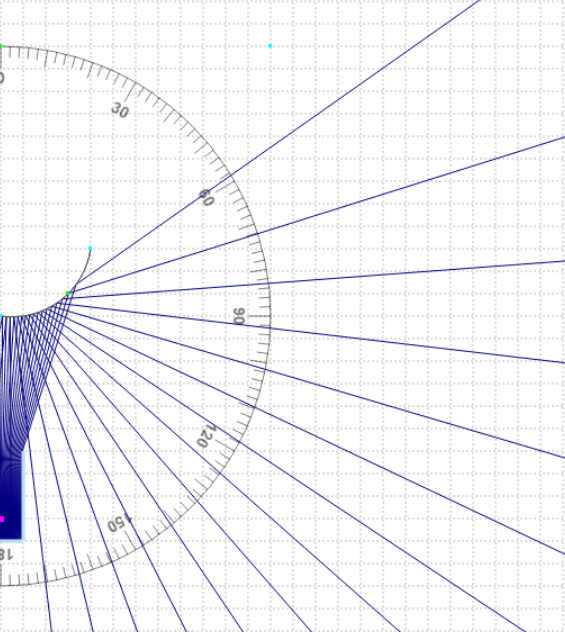
\includegraphics[width=0.6\textwidth]{Figures/sim_globe.PNG}
\caption{Simulation of transmitting with a globe shaped lens}
\label{fig:sim_globe}
\end{figure}

The spherical shaped lens in figure~\ref{fig:sim_globe} scatters the waves in a wide spread pattern.
The energy transmitted at an angle, with respect to the transmitter axis, greater than \SI{120}{\degree} does not reach the other Zebros.
This means a large part of the generated energy is lost as it's transmitted towards the Zebro body and not to the antenna of the other Zebros.
In conclusion the sphere produces an unfocussed radiation pattern.

\begin{figure}[H]
\centering
\begin{subfigure}{.5\textwidth}
  \centering
  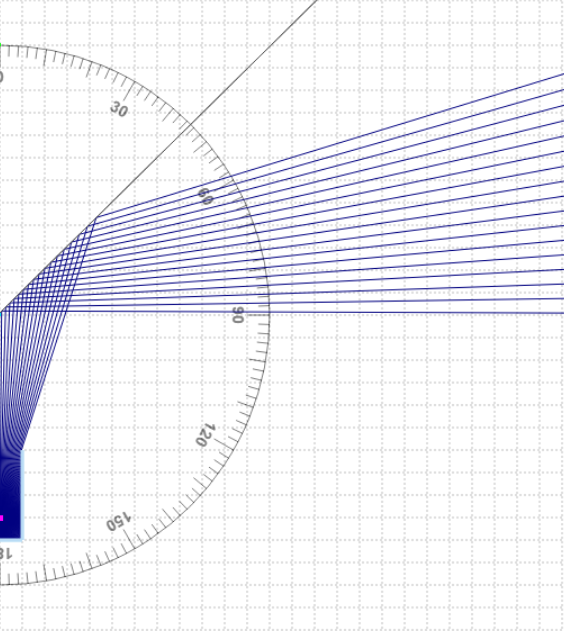
\includegraphics[width=0.85\textwidth]{Figures/sim_cone_45.PNG}
  \caption{45 degree cone}
  \label{fig:sim_cone_45}
\end{subfigure}%
\begin{subfigure}{.5\textwidth}
  \centering
  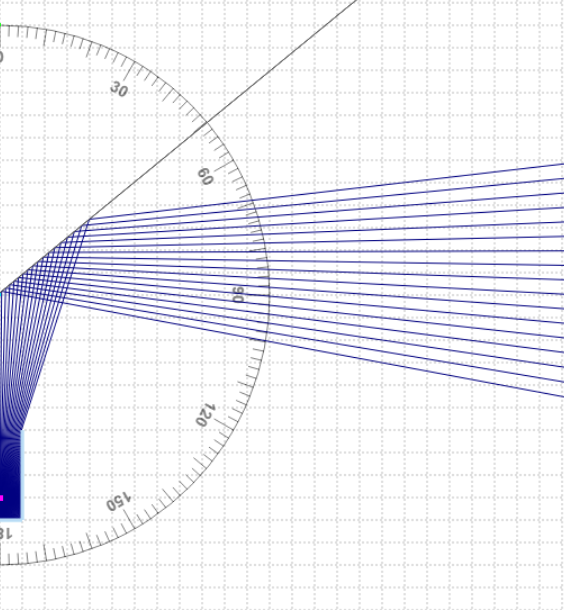
\includegraphics[width=0.9\textwidth]{Figures/sim_cone_50.PNG}
  \caption{50 degree cone}
  \label{fig:sim_cone_50}
\end{subfigure}
\caption{Simulation of transmitting with a cone shaped lens}
\label{fig:cone}
\end{figure}

%\begin{figure}[H]
%\centering
%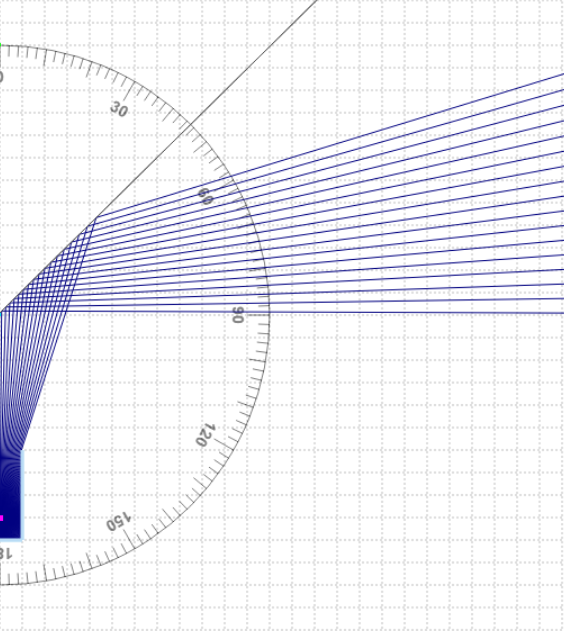
\includegraphics[width=0.6\textwidth]{Figures/sim_cone_45.PNG}
%\caption{Simulation of transmitting with a 45 degree cone shaped lens}
%\label{fig:sim_cone_45}
%\end{figure}

We see from figure~\ref{fig:sim_cone_45} that the cone produces a focussed beam.
In this case the beam is focused around \SI{75}{\degree} meaning that the energy is directed upwards instead of in the horizontal direction.

%\begin{figure}[H]
%\centering
%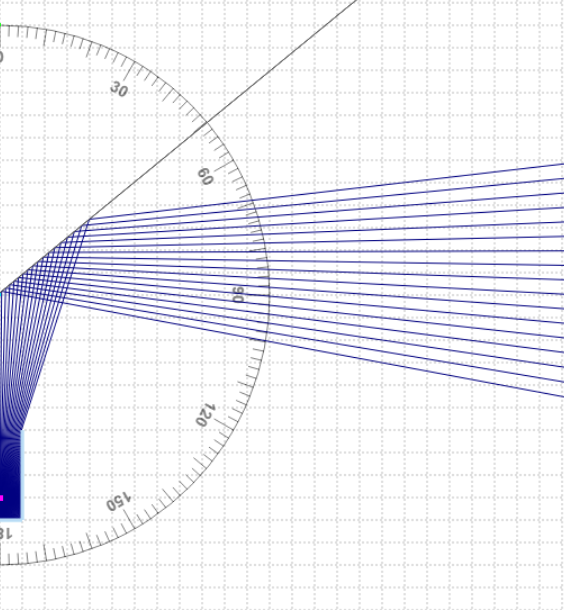
\includegraphics[width=0.6\textwidth]{Figures/sim_cone_50.PNG}
%\caption{Simulation of transmitting with a 50 degree shaped lens}
%\label{fig:sim_cone_50}
%\end{figure}

The \SI{50}{\degree} cone produces a beam focused around \SI{90}{\degree} as seen in figure~\ref{fig:sim_cone_50}.
In this case the energy is directed in the horizontal direction.

\begin{figure}[H]
\centering
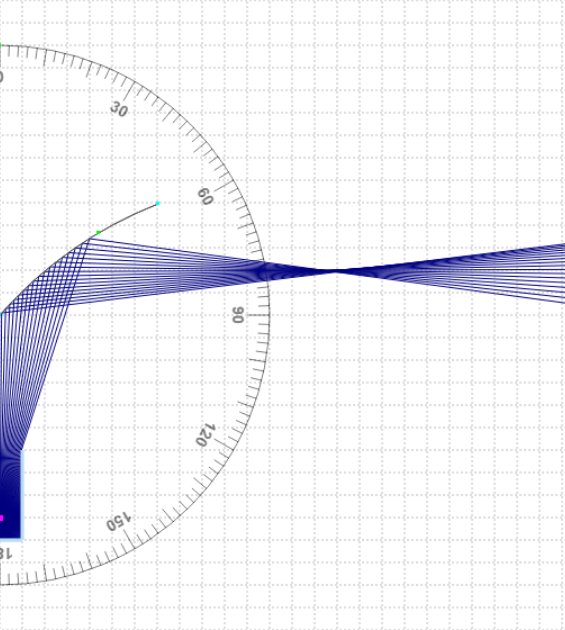
\includegraphics[width=0.6\textwidth]{Figures/sim_par.PNG}
\caption{Simulation of transmitting with a parabolic shaped lens}
\label{fig:sim_para}
\end{figure}

The parabolic antenna allows us the set a focal point for the beam as seen in figure~\ref{fig:sim_para}.
This would be ideal if the distance between Zebros is static so we could place the focal point on the antenna of the other Zebros.
In a moving swarm this Antenna has no advantage over the other shapes.

Comparing the simulation results shows us that for our situation, moving robots in the horizontal plane, the \SI{50}{\degree} cone antenna is the best option.

\begin{figure}[H]
\centering
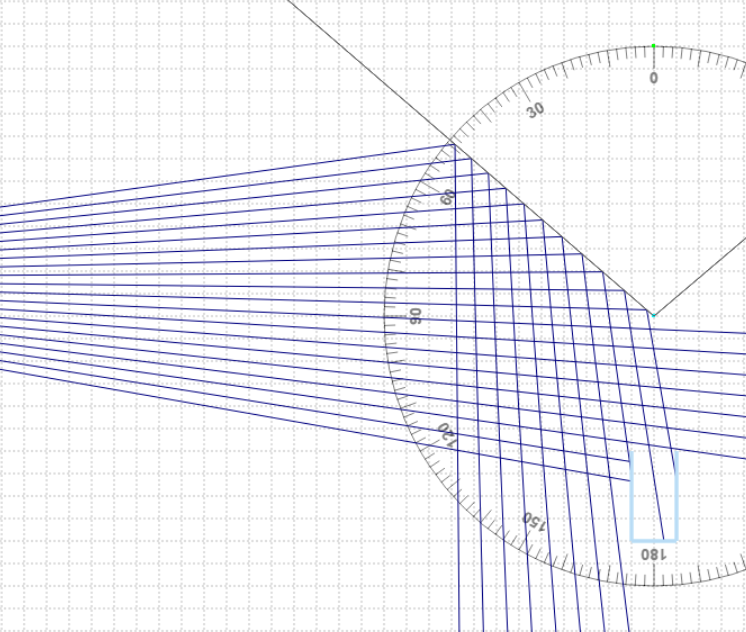
\includegraphics[width=0.6\textwidth]{Figures/sim_cone_rec.PNG}
\caption{Simulation of receiving with a \SI{50}{\degree} cone shaped lens}
\label{fig:sim_cone_rec}
\end{figure}

Figure~\ref{fig:sim_cone_rec} shows the receiving behaviour of the \SI{50}{\degree} cone when waves, reflected by another \SI{50}{\degree} antenna, are incident on the lens.
We see that the incident waves are reflected towards the transducer at the centre of the lens.
This means that the \SI{50}{\degree} antenna is both suitable for transmitting and receiving the ultrasonic pulse.

\subsection{Receiver circuit simulations}

In figure \ref{fig:simulationreceiver} are Falstad \cite{Falstad}
simulations visible of the receiver circuit discussed before in section \ref{chap:receivercircuit}. In the figure are 4 signals visible:

\begin{itemize}
\item
The green signal, the signal after the first stage of amplification
\item
The red signal, the signal after the second stage of amplification
\item
The orange signal, the signal after the peak detection circuit
\item
The pink signal, the $V_{th}$ of the first comparator stage
\end{itemize}

In figure \ref{fig:sim_receive} you see the operation amplifier signals of the receiver circuit. Between 0 and $0.075*10^{-1}ms^{-1}$ no ultrasonic signal is detected on the transceiver, between $0.075*10^{-1}$ and $0.525*10^{-1}ms^{-1}$ the ultrasonic transceiver receives a ultrasonic signal. And after $0.525*10^{-1}ms^{-1}$ the ultrasonic transceiver receives no ultrasonic pulse any more.
The signal received on the ultrasonic transceivers have an amplitude between the 0 and $100mV$. This signal is amplified in the first stage of the circuit, this is the green signal in figure \ref{fig:sim_receive}. The second stage amplification results in a signal with a higher amplitude, with a maximum amplitude of $4.5V$ due to the $4.5V$ put on the plus pin of the operational amplifier and the power source of $9V$. This signal is visible in the figure as the red signal.
The peak detection circuit charges a capacitor in this circuit, and discharges over a resistor. This results in the orange signal. This makes it possible to detect if there is an ultrasonic signal received. If the voltage of the peak detection signal is higher than the $V_{th}$, the pink signal, the comparator switches it's output. And if the peak detection signal becomes lower than the $V_{th}$ the comparator signal switches back. Both dan happen with a bit of delay since the capacitor needs to be charged or discharged. So the desired signal of the peak detection circuit needs to rise and fall fast, but not to fast otherwise the peak detection circuit won't work any more.\\

\begin{figure}[H]
\centering
\begin{subfigure}{.5\textwidth}
  \centering
  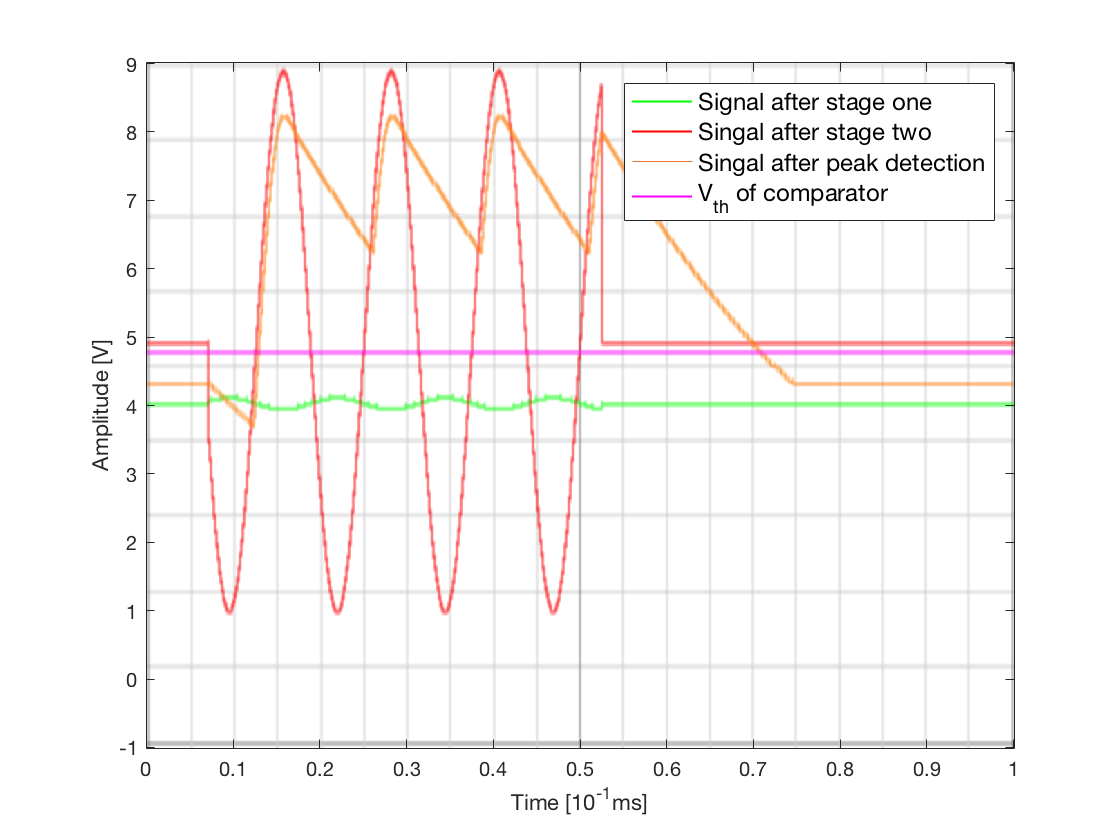
\includegraphics[width=1.0\textwidth]{Figures/receiver_simulations.PNG}
  \caption{Operation amplifier signals}
  \label{fig:sim_receive}
\end{subfigure}%
\begin{subfigure}{.5\textwidth}
  \centering
  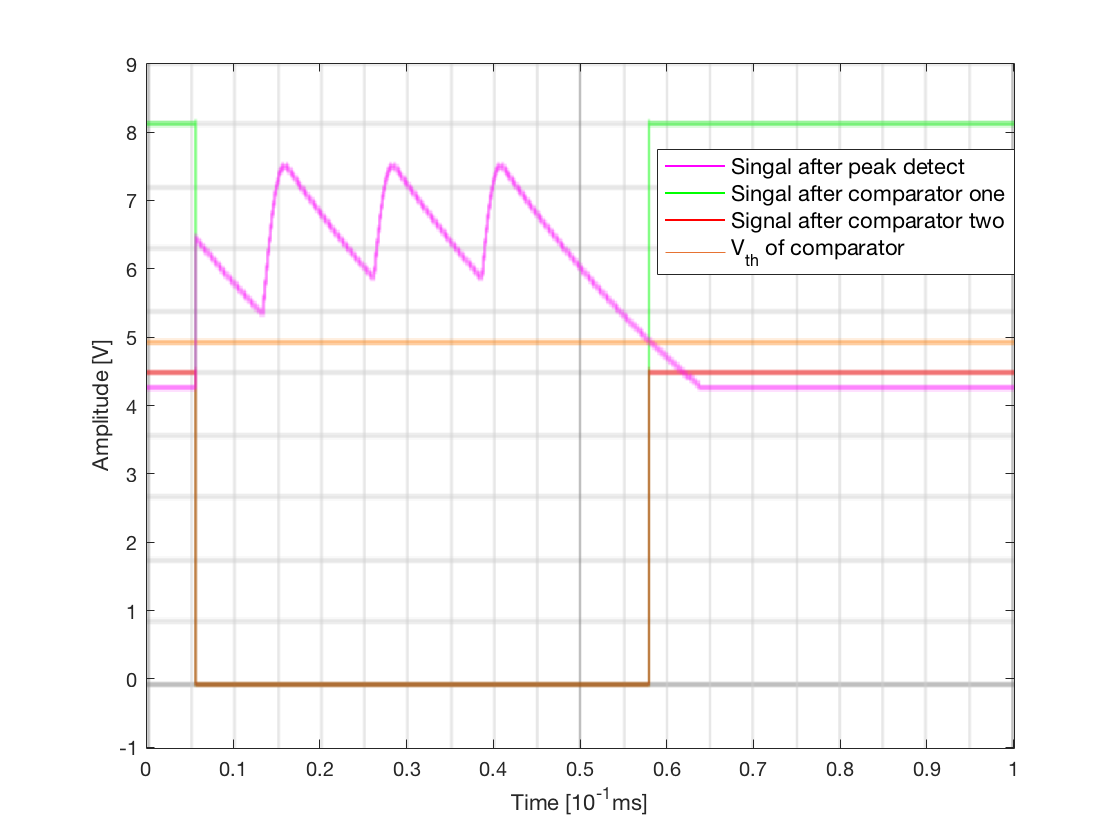
\includegraphics[width=1.0\textwidth]{Figures/receiver_simulations2.PNG}
  \caption{Comparator signal}
  \label{fig:sim_receive2}
\end{subfigure}
\caption{Simulation of receiver circuit}
\label{fig:simulationreceiver}
\end{figure}


In figure \ref{fig:sim_receive2} the signals of both comparator stages are visible, together with the peak detection signal and the $V_{th}$ of the first comparator. Again is no ultrasonic signal detected between 0 and $0.05*10^{-1}ms^{-1}$, and a signal detected between $0.05*10^{-1}ms^{-1}$ and $0.5*10^{-1}ms^{-1}$ and after $0.5*10^{-1}ms^{-1}$ no ultrasonic signal is detected any more.
The comparators switch when the peak detection signal becomes higher than $V_{th}$ and the other way around. The second comparator has a $V_{th}$ of $2.5V$, so switches together with the signal of the first comparator stage. This switching is between the desired 0 and $5V$ for the micro controller.


\section{Conclusion}
From the simulations done in this chapter we can conclude that the antenna we are going to use for the prototype will have a \SI{50}{\degree} cone, since the reflections of this cone have the best horizontal reflecting characteristics. And together with that have the best transmitting and receiving characteristics.  The transmitting circuit not discussed in this part of the thesis, this because the MIC4428 \cite{MIC4428} IC isn't available in simulation software, so testing in real life is the way we are going to test the transmitting part. The receiver circuit works as we wanted in the simulations so we are going to make this circuit on a prototype solder board and test it in real life.
